%THIS IS AN EXAMPLE OF HOW YOU MIGHT INTRODUCE A CHAPTER WHICH HAS ALREADY BEEN PUBLISHED.
\cleartoevenpage
\pagestyle{empty}	%Use this to suppress the header from the preceding chapter.

\noindent
%The following publication has been incorporated as Chapter~\ref{Chap:label}.

%\noindent
%1.~\cite{citationkey} \textbf{Your Name}, Co-author 1, and Final Author, \href{linktoyourpaper}{Title of your paper}, \textit{Journal} Issue, Number, Year

\begin{table}[h]
	\begin{center}
	\begin{tabular}{|c|l|l|}
		\hline
		Contributor & Statement of contribution & \% \\
		\hline
		\textbf{Your Name}				& writing of text 					& 70\\
															& proof-reading							& 60 \\
															& theoretical derivations 	& 70\\
															& numerical calculations 		& 100\\
															& preparation of figures 		& 80 \\
															& initial concept						& 10 \\
		\hline
		Co-author 1								& writing of text 					& 20\\
															& proof-reading							& 10 \\
															& supervision, guidance 		& 20\\
															& theoretical derivations 	& 10\\
															& preparation of figures 		& 20 \\
															& initial concept						& 10 \\
		\hline
		Final Author							& writing of text 					& 10\\
															& proof-reading							& 30 \\
															& supervision, guidance 		& 80 \\
															& theoretical derivations 	& 20 \\
															& preparation of figures 		& 10 \\
															& initial concept						& 80 \\
		\hline
	\end{tabular}
	\end{center}
\end{table}

%-------------------------------------------------------------------------------------------------------%
%-------------------------------------------------------------------------------------------------------%
%-------------------------------------------------------------------------------------------------------%
%-------------------------------------------------------------------------------------------------------%
%-------------------------------------------------------------------------------------------------------%
%-------------------------------------------------------------------------------------------------------%
%This is an internal chapter of the thesis.
%If you have a long title, you can supply an abbreviated version to print in the Table of Contents using the optional argument to the \chapter command.
\chapter[A description of the process biokinetics of phototrophic systems]{A description of the process biokinetics of phototrophic systems}
\label{Chap:chap2}	%CREATE YOUR OWN LABEL.
\pagestyle{headings}

This chapter is based upon work which has been published during the course of the PhD programme.\\

D. Puyol, \textbf{E. Barry}, T. H\"{u}lsen, and D. Batstone. A mechanistic model for anaerobic phototrophs
in domestic wastewater applications: Photo-anaerobic model (PAnM).
\textit{Water Research}, 116:241–253, 2017. Publisher: Elsevier Ltd.

\section*{Abstract}


\section{Introduction}
\label{Sec:chap2_intro}

The treatment of wastewaters is currently seeing a trend away from merely treating wastes to recapturing and reusing the energy and nutrients contained within the streams. Of increasing interest are photosynthetic and phototrophic organisms, such as microalgae \cite{Ward2014} and purple phototrophic bacteria (PPB) \cite{Hulsen2014} respectively. While both organisms can be used to partition organics and nutrients to a solid phase for reuse, PPB present an advantage in that they are able to recycle electrons during cyclic anoxygenic photosynthesis, meaning they can harvest and retain electrons, resulting in a higher energetic efficiency than that of algae. Photoconversion efficiencies are also higher for PPB at 6-8\% \cite{Miyake1987} than for algae at less than 5\% \cite{Posten2009}. Despite the numerous studies demonstrating use cases of PPB to produce bioplastics \cite{Melnicki2009} and treat wastewaters such as different meats, dairy and sugar \cite{Hulsen2018}, latex \cite{Kantachote2005}, and tofu \cite{Zhu1999}, the widespread adoption of these microorganisms has been slow. This is in large part due to several process limitations, such as photon conversion efficiency (or energy costs), solid-liquid separation issues for harvesting, and the requirements of extra readily biodegradable chemical oxygen demand (COD) in order to achieve discharge limits in nitrogen and phosphorus \cite{Hulsen2015}.

Process modelling can be used to address the aforementioned issues, as well as to better understand and optimise phototrophic systems. A suite of modelling work already exists for PPB under different conditions for varying levels of abstraction. Previous low-level modelling efforts involved the description of PPB metabolism based on the electron transport chain within a complex network of metabolic processes \cite{Golomysova2010}. These models are necessary for a deeper understanding of the cell processes of a variety of PPB, however they can not easily be implemented in a process modelling framework to be used within a broader industrial-scale model. Much work has been done on the production of hydrogen from PPB \cite{Eroglu2008}. Key cell processes for hydrogen producing PPB are photoheterotrophic growth, with chemoheterotrophic and photoautotrophic growth described as well. The processes involved are similar to those for wastewater treatment and related applications, however extra processes in wastewater treatment such as biomass decay and hydrolysis and fermentation must also be described. Despite the rich body of modelling knowledge, there currently exists no process-level wastewater models which can be used as modules in broader process modelling environments, similar to the International Water Association (IWA) family of models \cite{Henze1987} such as the Anaerobic Digestion Models (ADM) \cite{Batstone2002}, or the Activated Sludge Models (ASM) \cite{Gujer1999}. 

This study evaluates the main biochemical processes of a PPB system with the aim of developing a mechanistic model to assess the modes of growth over batch and continuous operation. The model describes photoheterotrophic, chemoheterotrophic, and photoautotrophic modes of growth, as well as the hydrolysis of particulate composites to readily biodegradable COD and the decay of PPB biomass. The model has been developed for a mixed culture system and has been written such that it can be adapted to be included in broader modelling environments, and the model can easily be extended or simplified. 

%-------------------------------------------------------------------------------------------------------%
%-------------------------------------------------------------------------------------------------------%
%-------------------------------------------------------------------------------------------------------%

\section{Materials and methods}
\label{Sec:chap2_mm}

\subsection{Model description}
The model has been developed to be compatible with the IWA, ASM and ADM families of models. As such, the units used in this particular study are presented in $\mathrm{g COD\, m^{-3}}$ for soluble and particulate organic matter, $\mathrm{g NH_4\mbox{-}N\, m^{-3}}$ for inorganic nitrogen, $\mathrm{g PO_4\mbox{-}P\, m^{-3}}$ for inorganic phosphorus, and $\mathrm{mol C\, m^{-3}}$ for inorganic carbon. Semi-mechanistic Monod kinetics have been used for all growth terms and limiting expressions, and the hydrolysis and decay processes have been assumed to follow first order kinetics. Inhibitory processes follow non-competitive inhibition. While this model describes a mixed culture system, few differences in behaviour between PPB have been observed \cite{Hulsen2016}. As such, a single PPB term has been chosen to represent all phototrophic microorganisms. 

\subsubsection{Modes of growth}
\noindent\textit{Photoheterotrophic growth}\par
\noindent This has been divided into two subcategories: growth on acetate ($\mathrm{S_{AC}}$), and growth on other organics ($\mathrm{S_S}$). Acetate uptake is represented separately due to differences in rates during experiments. The growth rate on acetate is roughly double that on other organics due to the the imbalance in carbon oxidation state between acetate and biomass. This process produces positive $\mathrm{CO_2}$. Photoheterotrophic uptake has been lumped for all other organic substrates due to similar behaviour as a result of similar substrate-biomass oxidation states. The organic substrates include volatile fatty acids, alcohols and sugars. Unlike acetate uptake, PPB growth in this lumped substrate results in consumption of $\mathrm{CO_2}$. Both processes occur in the presence of infra-red radiation, with heterotrophic growth through the tri-carboxylic acid cycle (TCA) assumed as the dominating pathway. \\


\noindent\textit{Photoautotrophic growth}\par
\noindent This process also requires infra-red radiation and is dominant in the absence of organic soluble substrates. This process uses inorganic compounds, excluding water, as its electron donor. Such electron donors include Fe$^{2+}$, sulfide, sulfate and hydrogen. Due to the minimal concentrations of sulfur and iron compounds in domestic wastewater, they have been omitted from the model and only $\mathrm{H_2}$ is used as an electron donor. \\

\noindent\textit{Chemoheterotrophic growth}\par
\noindent In the absence of infra-red radiation, chemoheterotrophic growth dominates. It involves the assimilative uptake of organics through fermentation or anaerobic oxidation processes. Acetate and $\mathrm{H_2}$ are products of this process, with $\mathrm{H_2}$ being used as an electron donor for photoautotrophic growth. Acetate does not undergo further oxidation in this process due to the lack of terminal electron acceptors in domestic wastewater \cite{Finneran2003}.\\

\noindent\textit{Cell decay}\par
\noindent Upon PPB cell decay, ammonium, phosphate, and inorganic carbon are released and PPB biomass is converted into biodegradable organic particulates ($\mathrm{X_S}$). \\

\noindent\textit{Hydrolysis and fermentation of particulates}\par
\noindent These processes have been lumped together and labelled as hydrolysis. This process involves biodegradable particulates decomposing into soluble organics, namely $\mathrm{S_S}$ and $\mathrm{S_{AC}}$, key nutrients, hydrogen and organic carbon. This process also includes the release of soluble and particulate inert matter ($\mathrm{S_I}$ and $\mathrm{X_{I}}$ respectively). \\

\noindent\textit{Treatment of acidity and temperature}\par
\noindent An ideal pH model has been implemented in the model in a similar fashion to the ADM1 model \cite{Batstone2002}. The implementation includes phosphate acid-base pairs with no ion pairing. This is sufficient for domestic wastewater, but for streams with extreme pH, high levels of pollutants, or for implementation in a more generic benchmark simulation framework, this model should be extended to include strong acids and bases. Temperature has not been included as a term in either the pH model or in the PAnM, but van't Hoff and Arrhenius expressions can be implemented for important parameters as previously investigated \cite{Hulsen2016a}. \\

\noindent\textit{Summary presentation of the model}\par
\noindent The temporal evolution of species follows general equation Eq.~\eqref{eq:base_ode} with state variable $\mathrm{\phi_i}$ where $\mathrm{\phi_i\, = \, \{S_{AC},\, S_S,\, S_{IC},\, S_{H_2},\, S_{IN},\, S_{IP},\, S_{I},\, X_{PB},\, X_{S},\, X_{I}\}}$. Soluble species are denoted by an $\mathrm{S}$ and particulate species are denoted by an $\mathrm{X}$.

\begin{equation}
    \label{eq:base_ode}
    \frac{d\phi_i}{dt} \, = \, \mathfrak{R}_i
\end{equation}

where $\mathfrak{R}_i$ is the rate of formation (positive) or consumption (negative) of species $\mathrm{\phi_i}$. The presentation and explanation of all species and their formation or consumption terms are best summarised in a Petersen matrix (Table~\ref{tab:petersen}).

 \begin{sidewaystable}[tp]
    \caption{Petersen matrix for the PAM-1 model for domestic wastewater treatment by purple phototrophic bacteria.}
    \label{tab:petersen}
    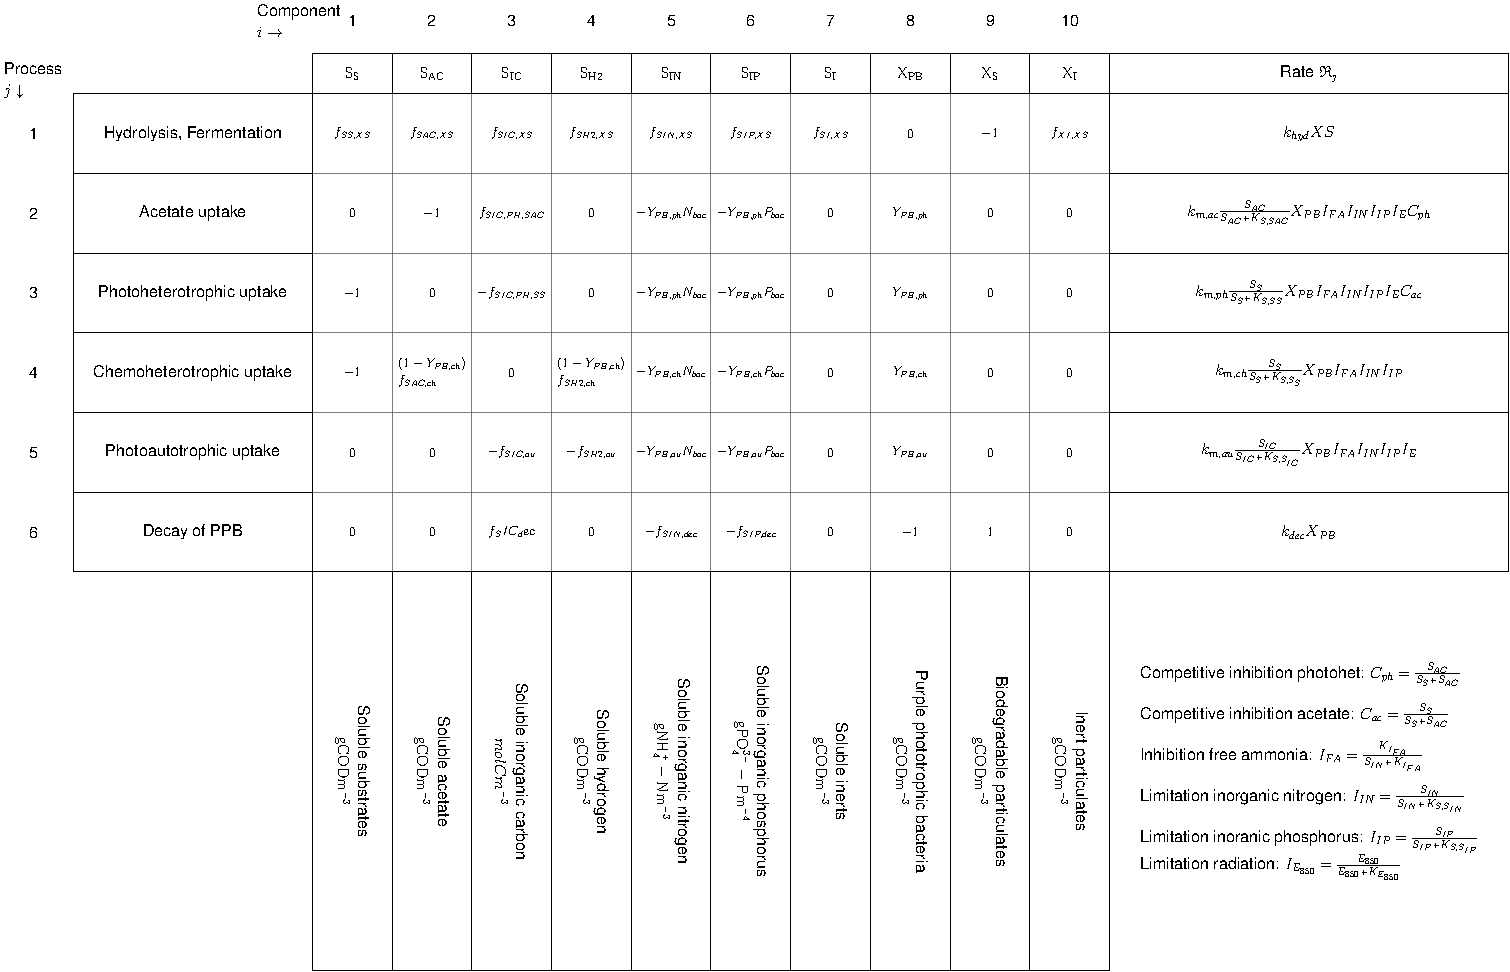
\includegraphics[width=1\linewidth]{Tables/petersen/petersen.pdf}
\end{sidewaystable}

\subsubsection{Integration with ASM models and ADM1}
Each component in the PAM-1 model can be translated into the family of IWA models. The organic compounds in this model can be transformed to ASM organic substrate by combining the acetate and other soluble organics fields. For organic particulates, $\mathrm{X_S}$ are the same for both ASM models and PAM-1. For soluble organics, $\left(S_S + S_{AC}\right)_{PAM1} \rightarrow \left(S_S\right)_{ASM}$. This quantity can then be translated to ADM1 through a model translation interface \cite{Nopens2009}. Both biodegradable and inert particulates, as well as inert solubles have direct analogues in both ASM and ADM1 models. Phototrophic biomass can be converted to ADM1 via the following relationship, $X_{PB} \rightarrow \left(aX_{ch} + bX_{li} + cX_{pr} + dX_I \right)$. The coefficients $a$, $b$, $c$, and $d$ are determined through the nutrient and COD ratios of the biomass, which have been determined experimentally \cite{Hulsen2014}. For inorganic nitrogen, $\left(S_{IN}\right)_{PAM\mbox{-}1} \rightarrow \left(S_{nh} + S_{no}\right)_{ASM}$. There are no changes for PAM-1 to ADM1 conversions of ammonium. To convert inorganic phosphorus, $\left(S_{IP}\right)_{PAM\mbox{-}1}$ can be expressed as either $\left(S_{IP}\right)_{ADM1}$ or $\left(S_{PO_4\mbox{-}P}\right)_{ASM2d}$. Inorganic carbon in both PAM-1 and ADM1 are expressed in the same manner, and $\left(S_{IC}\right)_{PAM\mbox{-}1}$ can be transformed into alkalinity in ASM as per the ADM/ASM model interface \cite{Nopens2009}.

\subsection{Experimental procedure}
Parameters were identified through a series of batch tests. The inoculum was sourced from a 2 L photoanerobic membrane bioreactor (PAnMBR) with steady-state operation of over 300 d \cite{Hulsen2016}. Domestic wastewater was sourced as feed for the PAnMBR and was collected from the Taringa and St. Lucia wastewater stations (Brisbane, Australia). The average strength of wastewater over the period was 572 $\mathrm{g COD m^{-3}}$ total COD and 241 $\mathrm{g COD m^{-3}}$ of soluble COD. There were 63 $\mathrm{g N m^{-3}}$ and 9 $\mathrm{g P m^{-3}}$ for ammonium and phosphorus respectively. In tests where wastewater was not used, synthetic Ormerod medium was used as per the batch tests carried out in previous studies \cite{Hulsen2014}. 

All batch tests for metabolic growth were done in 100 mL volumes in 160 mL serum flasks. The tests were carried out in triplicate. Once the flasks were inoculated and dosed, they were flushed with $\mathrm{N_2}$ to remove oxygen from the headspace. All experiments were done at $\mathrm{20 \, \degree C}$ in an orbital shaker at 150 rpm (Edwards Instrument Company). The flasks were irradiated with 150 W lamps and the UV and visible parts of the spectrum were filtered out using photo foil as described in previous batch experiments \cite{Hulsen2014}. Blank samples with zero substrate were included in all metabolic experiments.

For hydrolysis and decay tests, the inoculum was collected in the same manner. Biomass were centrifuged in 50 mL Falcon tubes at 3750 rpm, with the pellet resuspended in 0.2 M NaCl. The centrifugation/resuspension process was done three times. The biomass was then placed in 500 mL of 0.2 M NaCl and was then redistributed into 2 250 mL Schott bottles. The bottles were flushed, placed on magnetic stirrers at 200 rpm for 30 days of operation. In order to analyse hydrolysis, aluminium foil covered one of the bottles so that no phototrophic growth would occur. Samples were taken twice-weekly for COD, VFA, $\mathrm{NH_4\mbox{-}N}$, $\mathrm{PO_4\mbox{-}P}$, total inorganic carbon (TIC), and pH. Headspace measurements were taken at the same interval for $\mathrm{CH_4}$, $\mathrm{H_2}$, $\mathrm{CO_2}$. Total suspended solids (TSS) and volatile suspended solids (VSS), as well as total Kjeldahl nitrogen (TKN) and total phosphorus (TP) were sampled and analysed every 7 days. The decay test was done with the same irradiance as that used in the metabolic growth tests. Measurements were made for TSS, VSS, TKN and TP and were taken every 7 days to monitor biomass decay. The test was done with 100 $\mathrm{g COD m^{-3}}$ of acetate and 10 $\mathrm{g N m^{-3}}$ of ammonium. 

Specific phototrophic activities were determined by both non-linear regression, and linear regression of biomass-normalised substrate concentration within a region of maximum consumption. All conditions for batch tests are summarised in Table \ref{tab:batch}. The HEPES buffer system was dosed at 5.9 g L\textsuperscript{-1} and the phosphate buffer contained 0.9 g K\textsubscript{2}HPO\textsubscript{4} and 0.66 g KH\textsubscript{2}PO\textsubscript{4}. The carbon sources are presented in gCOD m\textsuperscript{-3} and the electron donor for photoautotrophy is presented in g m\textsuperscript{-3}. 

\begin{table}[tp]
    \centering
    \small
    \renewcommand{\arraystretch}{1.4}
    \caption{Batch conditions for metabolic tests}
    \tabcolsep=0.11cm
    \begin{tabular}{@{}p{3cm} p{1.4cm} p{1.5cm} p{1.7cm} p{1.4cm} p{1.4cm} p{1.4cm} p{1.4cm} p{1.4cm}@{}} \toprule
        Mechanism & Medium & Buffer system & COD:N:P\textsuperscript{**} & C source & Electron donor & Electron acceptor & Positive control & Negative control\\
        \hline
        Photoheterotrophy & Ormerod& HEPES & 100:10:2 & Acetate (130), propionate, butyrate, ethanol (100) & Organic & CO\textsubscript{2}&  $\mathrm{1\, g}$ NaHCO\textsubscript{3} added&  -- \\
        
        Nitrogen limitation & Ormerod&  HEPES & 100:1.4:2& Acetate (130) & Organic & CO\textsubscript{2}& No limitation & -- \\
        
        Phosphorus limitation & Ormerod & HEPES & 100:10:0.15 & Acetate (130) & Organic & CO\textsubscript{2}& No limitation & -- \\
        
        Photoautotrophy & Ormerod & Phosphate & 100:20:$\infty$ & NaHCO\textsubscript{3} (140\textsuperscript{*}) & Na\textsubscript{2}S (300)& CO\textsubscript{2}& -- & No Na\textsubscript{2}S \\
        
        Chemoheterotrophy & Ormerod & HEPES &100:10:2 & Ethanol (60), Acetate (130) & Organic& Acetate& + light& -- \\
        
        Inhibition of $\mathrm{H_2}$ production & 
        Ormerod & Phosphate & 100:15:$\infty$&Acetate (600) & Organic & CO\textsubscript{2} & --  & N limitation (1/10) \\
        ---\texttt{"}---& DWW & -- & 100:12:4 &DWW (278) & Organic & CO\textsubscript{2}&-- &Acetate (600) \\
        \bottomrule
    \end{tabular}
    \footnotesize
    \begin{tabular}{@{}p{4cm} p{10cm}}
        \textsuperscript{*}Units are gC m\textsuperscript{-3} & \textsuperscript{**} $\infty$ means excessive concentration due to buffer \\
    \end{tabular}
    \label{tab:batch}
\end{table}

\subsection{Analytical methods}
Total and soluble COD (TCOD and SCOD respectively) were determined by COD cell tests (Merck, 1.14541.0001, Darmstadt, Germany). Dissolved $\mathrm{NH_4\mbox{-}N}$ and $\mathrm{PO_4\mbox{-}P}$ were measured by a QuikChem8000 Flow Injection Analyser (FIA) (Hach Company, Loveland, USA). Temperature and pH were measured using an Oakton pH 11 Series (Vernon Hill, Illinois, USA). Determination of TSS and VSS was done by filtration. The samples were filtered with a known volume of biomass suspension, dried in an oven at 105 $\pm$ 2 $\degree$C for 24 hours and weighed for TSS. For VSS, the same sample was then placed in a furnace at 550 $\pm$ 5 $\degree$C for 2 hours \cite{APHA1998}. The incident irradiance ($\mathrm{Wm^{-2}}$) was measured with an infra-red sensor (PAS Port\texttrademark, Roseville, California, USA). VFA samples were analyzed by gas chromatography (Agilent Technologies 7890A GC System, Santa Clara, California, USA) equipped with a flame ionization detector (GC/FID) and a polar capillary column (DB-FFAP). Gas samples were analyzed by GC (2014 Shimadzu, Kyoto, Japan) with thermal coupled detector \cite{Tait2009}. TKN and TP were determined using sulfuric acid, potassium sulfate and copper sulfate catalyst in a block digester (Lachat BD-46, Hach Company, Loveland, CO, USA) \cite{Patton1992}. TIC was analyzed by using a total organic carbon (TOC) analyzer (Shimadzu TOC-L CSH TOC Analyzer with TNM-L TN unit) coupled to a near infrared detector (NIRD) for measuring the CO2. All soluble constituents were determined after filtering with a 0.45 mm membrane filter (Millipore, Millex\textsuperscript{\textregistered}-HP, Merck Group, Darmstadt, Germany).

\subsection{Data analysis}
\subsubsection{Data handling}
The concentration of phototrophic biomass was calculated from the method for determining VSS. The biomass was then converted to a COD quantity by the molecular formula CH\textsubscript{1.8}O\textsubscript{0.38}N\textsubscript{0.18} \cite{Mckinlay2010}. This gave 1.78 kg COD for 1 kg biomass as VSS. Biomass yields were calculated from initial and final biomass concentrations based on the consumption of substrate during the batch tests. The yields (in concentration of VSS) were then converted to COD and expressed as unitless quantities (kgCOD\textsubscript{PPB} kgCOD\textsuperscript{-1}). 

\subsubsection{Statistical analyses and uncertainty analysis}
When samples were measured to be outside of the range of calibration for a given test, the measurements were repeated by dilution of the samples. Internal or external standards were used for all measurements. Calibration of all measurement equipment was done at least once per week. All parameters were estimated from triplicate samples by with the minimisation of the cost function (J) chosen as residual sum of squares Eq. \eqref{eq:cost_function}.
\begin{equation}
    \label{eq:cost_function}
    \underset{\Theta}{\mathrm{min}}\, \, \mathrm{J}(\Theta)\quad  = \quad \sum_{i = 1}^{n\in\mathbb{N}} \left(y_i - \hat{y}(\Theta)_i    \right)^2
\end{equation}

where $\Theta$ is the set of parameters that must be found such that the squared distance between the experimental data points $y_i$ and the hypothesised model $\hat{y}_i$ is minimised. For multiple parameter optimisation, the value of J was set to a critical J value (J\textsubscript{crit}) based on the F statistic determined by the number of parameters of interest, the number of data points and the significance threshold (here 95\%). \cite{Batstone2003}. Uncertainty in parameters was determined from their standard error and a two-tailed Student t-test (5\% threshold). All determined parameters are expressed in terms of 95\% confidence intervals. The error bars in experimental data represent 95\% confidence intervals in mean based on a two-tailed t-test. The uncertainty of the slope when determining specific phototrophic activities was done using the Microsoft Excel 2013 Regression tool and was rechecked using the Scipy Stats package \cite{Scipy2001}. Unless otherwise stated, all statistical analyses were done with a 5\% significance threshold.

\subsection{Simulations of PAM-1}

\subsubsection{Simulation of a phototrophic batch system}
The model was tested to explore different scenarios in order to understand the limits of the process and to highlight the possible adaptations of he model by biomass shifts on metabolism. The model was implemented using SciPy \cite{SciPy2001} and NumPy \cite{NumPy2011} for numerical functionality, and Matplotlib \cite{Hunter2007a} for visualisation of results. A series of three simulations were done on a PAnMBR system.

The first simulations were designed to assess the effects of limiting substrate concentrations on the uptake of other substrates. A range of inorganic nitrogen initial concentrations (0 gN m\textsuperscript{-3} to 50 gN m\textsuperscript{-3}) and SCOD (S\textsubscript{S} + S\textsubscript{AC}) ranging from 0 gCOD m\textsuperscript{-3} to 800 gCOD m\textsuperscript{-3} (equally divided) were simulated with all other substrates in excess. The same simulation was done for inorganic phosphorus where the range of initial concentrations was from 0 gP m\textsuperscript{-3} to 12 gP m\textsuperscript{-3} and the same initial concentrations for SCOD. 

The second simulations were designed to examine the effect of dark/light cycles on PPB metabolism under low and high rates of chemoheterotrophic activity (k\textsubscript{M,ch} = 0.074 and 0.7 d\textsuperscript{-1} respectively). The light/dark cycling were toggled for a duration of 12 hours at a time over a simulated period of two days. 





\subsubsection{Simulation of a phototrophic continuous system}
The resulting kinetic expressions were used in the development of a continuous PAnMBR model. The concentration of bioavailable SCOD in medium strength wastewater was insufficient for the system to achieve TN and TP discharge limits \cite{Hulsen2016}. To achieve full removal, additional SCOD was required. The goals of the simulation were the following: a) to highlight the requirement of additional SCOD to achieve total nutrient removal, and b) to demonstrate that the inclusion of a primary clarifier can lead to an organic sludge enriched in PPB biomass. Dynamic influent data was simulated according to an influent generator model \cite{Gernaey2011}, and adapted to the typical concentrations of primary influent previously reported \cite{Hulsen2014}. Based on the average influent characteristics and an hydraulic retention time (HRT) of 12 h, volumetric loading rate (VLR) of 400 $\pm$ 12 gCOD m\textsuperscript{-3} d\textsuperscript{-1} and a solids retention time (SRT) of 3 d, a reactor volume of 70 m\textsuperscript{3} was applied. An ideal primary clarifier was included, with a solids removal efficiency of 60\% $\pm$ 3\% \cite{Tchobanoglous}. The generation of realistic influent was done in Simulation and subsequent data processing were done in Matlab Simulink (MATLAB R2015a, The MathWorks Inc., Natick, MA) and the simulations and data processing were done using SciPy, NumPy and Matplotlib in Python 3 \cite{Scipy2001, NumPy2011, Hunter2007a}. The \texttt{odeint} subroutine was sufficient for solving the stiff system of differential equations. The case was simulated for 609 days with 3 stages of differing SCOD concentrations. The dynamic influent after settling was applied directly during Stage I until day
300. During Stage II (days 300-450), acetate was added to the optimum COD:N:P ratio of 100:7.1:1.8 (calculated in the Jupyter notebook) based on the limiting nutrient (N or P). During Stage III, acetate addition was ceased. This was to assess process response to a sudden change, and to demonstrate that the system requires wastewater with a specific COD/N/P ratio. State equations were implemented in a fixed volume, completely mixed membrane bioreactor. The results from the simulation were balanced over COD, N, P and C. The simulation has been packaged into a Jupyter notebook at \textbf{Gitlab Release for PAM notebook}.

\section{Results and discussion}
Inoculum for all experiments cam from a lab-scale photo-anaerobic membrane bioreactor. Most organisms are related with $\alpha$\textit{-proteobacteria}, PPB accounting for greater than 70\% of gene copies detected by pyrosequencing. \textit{Rhodobacter sphaeroides} accounts for more than 60\% of the microbiota \cite{Hulsen2016}. Other photosynthetic organisms accounted for less than 1\% of the total gene copies, meaning that photosynthetic or phototrophic biomass was mostly PPB. 

\subsection{Growth processes}

\subsection{Batch simulations}

\subsubsection{Limiting N, P and SCOD}




\subsubsection{Light/dark cycling}

\begin{figure}[tp]
    \centering
    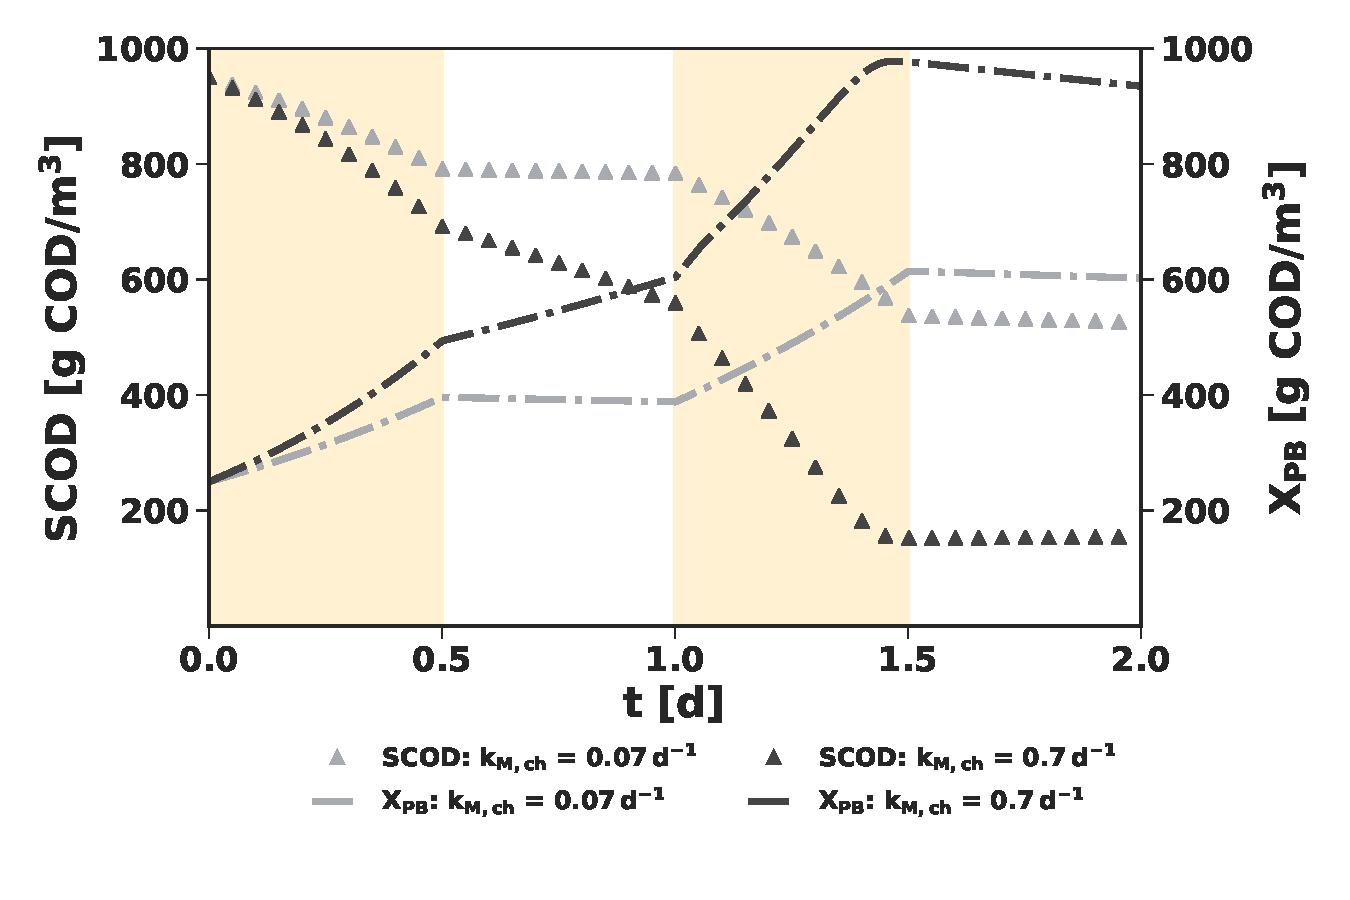
\includegraphics[width=1\linewidth]{./Chap2/simulations/ch2_kmch.pdf}
    \caption{Effect of dark/light cycling on PPB metabolism under low (light colour) and high (dark colour) chemoheterotrophic activity. There is an order of magnitude difference between the activities. A full light/dark cycle is a 24 hour period to mimic perceived solar irradiance in an outdoor photobioreactor.}
    \label{fig:ch2_kmch}
\end{figure}

\subsubsection{Sensitivity of specific photoautotrophic uptake activity}


\subsection{Continuous simulations}




\section{Conclusions}

%\begin{instructional}
%Add your text here. Use \verb|\cite| to add citation labels. Reference sections, tables, and figures using \verb|\ref|. Use %\verb|\eqref| for equations. The `section' symbol $\S$ is obtained using \verb|$\S$|. Figures and other floats are added using their %respective environments. Use \verb|\longtable| to split tables over page.
%\end{instructional}
